\section{Official-data calibration and numerical experiments}

\subsection{Pre-registered calibration}

The design was frozen before results under identifier
CRR-ISSUE34-FULL-MODEL-2026-07-27, with design hash
\texttt{\DesignHash}. Kansas was selected because corn, soybean and winter
wheat have complete public observations in every 2016--2024 analysis year and
form a relevant diversified crop set. The 2016--2023 observations calibrate
the score and margins; 2024 is excluded from the score and retained for
external evaluation.

The score for crop \(i\) is the mean of Kansas yield divided by same-year
national NASS yield over 2016--2023. It measures relative historical yield
potential, not revenue. Scores are \ScoreCorn{} for corn, \ScoreSoy{} for
soybean and \ScoreWheat{} for winter wheat. Real per-acre margin combines
Kansas yield, national harvest price, national operating cost and CPI-U
conversion to 2024 dollars. Mean margins are \(\$\,\MarginCorn\),
\(\$\,\MarginSoy\) and \(\$\,\MarginWheat\), respectively. These aggregate
inputs are transparent calibration values, not farm-level profits.

The primary marginal law is Student-\(t\) with five degrees of freedom. The
primary joint law is a Student-\(t\) copula with four degrees of freedom and
Kendall's \(\tau=0.25\), simulated with 512 optimization scenarios.
Sensitivity uses Gaussian and empirical-quantile margins; Gaussian,
Student-\(t\) and Clayton copulas; and \(\tau\in\{0,0.15,0.30,0.45,0.60\}\).
The eight annual observations cannot estimate extreme tails precisely, so
these are registered structural stress paths rather than fitted farm copulas.

Land is normalized to one. Crop lower bounds are 0.05, 0.10 and 0.05; upper
bounds are 0.55, 0.65 and 0.60. The operating budget is \(\$330\), corn is
capped at 0.50 by rotation, soybean has a 0.10 contract minimum, and planting
labour and harvest equipment have shared crop-specific coefficients. The
primary confidence level is 0.95 and risk tolerance \(\rho=0.5\). All
counterfactuals use the same full constraint system unless a constraint is the
registered sensitivity dimension.

\subsection{Primary reversal}

The expected-profit endpoint without loss-CVaR assigns 0.280 to corn, 0.650
to soybean and 0.070 to winter wheat. It strongly reverses but has loss-CVaR
\(\$\,\PrimaryNoRiskCVaR\), exceeding the primary risk ceiling. The
minimum-CVaR endpoint attains \(\$\,\PrimaryMinCVaR\) but sacrifices expected
profit. The registered midpoint ceiling is \(\$\,\PrimaryCVaR\).

The full optimum assigns \PrimaryCorn{} to corn, \PrimarySoy{} to soybean and
\PrimaryWheat{} to winter wheat. The highest-ranked crop therefore receives
the least land, a strong selected reversal involving both pairs. The land and
CVaR restrictions bind; idle land is zero. Expected profit is
\(\$\,\PrimaryProfit\) per normalized acre and realized finite-scenario
loss-CVaR equals the ceiling to numerical precision. Maximum primal,
stationarity and complementarity residuals are \(\KKTPrimal\),
\(\KKTStationarity\) and \(\KKTComplementarity\), respectively.

This result has two related but distinct causes. The score--margin separation
favours soybean economically even though winter wheat ranks agronomically
first. The CVaR ceiling prevents the unconstrained expected-profit corner and
requires a less concentrated allocation. Operational constraints delimit the
available path between those endpoints. Reversal is thus not attributed to
one scalar mechanism by inspection; it is the outcome of the declared model
and active-set geometry.

\subsection{Conditional phase diagram}

Figure~\ref{fig:phase} reports all \PhaseCells{} combinations of copula
family, Kendall's \(\tau\) and risk tolerance. Reversal occurs in
\PhaseReversal{} cells and is strong in \PhaseStrong. There are no infeasible
cells, but two Clayton cells have multiple optima. Most reversal regions are
connected on the registered grid; Clayton at \(\tau=0.30\) is disconnected.
The first selected-reversal index ranges from 0 to 0.3 across family and
dependence paths, while the first strong-reversal index can be as high as 0.9.

The nonmonotonic cells are substantively important. Increasing dependence can
change which resource or risk constraint binds, and that active-set transition
can move individual crop shares in either direction. The phase diagram
therefore supports Proposition~\ref{prop:convexorder}'s feasible-set logic
without claiming coordinate monotonicity. Scalar lower-tail dependence is
reported as a diagnostic within each family, not used as a cross-family
ordering statistic.

\begin{figure}[t]
\centering
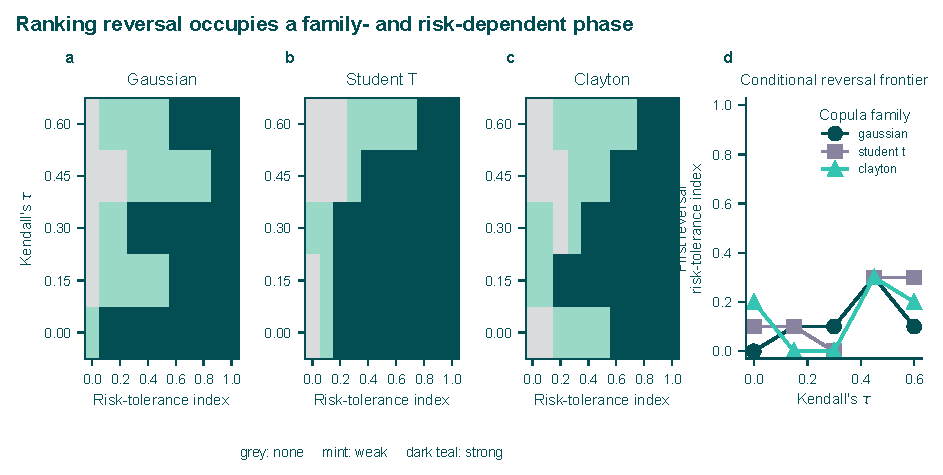
\includegraphics[width=\textwidth]{figures/issue34/Figure2.pdf}
\caption{\textbf{Ranking reversal occupies a family- and risk-dependent
phase.} \textbf{a--c}, Classification across risk tolerance and Kendall's
\(\tau\) for Gaussian, Student-\(t\) and Clayton copulas. Grey indicates no
reversal, teal weak reversal and red strong reversal. \textbf{d}, The first
selected-reversal risk tolerance varies non-monotonically across the named
family paths. All \PhaseCells{} registered cells, including \PhaseMultiple{}
multiple-optimum cells, are retained.}
\label{fig:phase}
\end{figure}

\subsection{Diversification failure under matched rank dependence}

The mean--variance benchmark and tail-aware model use the same marginal
means and standard deviations and matched Kendall's \(\tau=0.25\). The
Student-\(t\) law nevertheless has lower-tail coefficient
\LowerTailCoefficient, whereas the Gaussian copula has zero asymptotic
tail dependence. The Gaussian mean--variance policy assigns 0.280, 0.650 and
0.070 to corn, soybean and winter wheat. Under the Student-\(t\) evaluation
law, its loss-CVaR is \(\$\,\DiversificationGaussianCVaR\), worse than and
above the registered ceiling \(\$\,\DiversificationRiskCeiling\). The
tail-aware policy attains \(\$\,\DiversificationTailCVaR\) and changes the
allocation.

All components of the executable failure criterion are met: the conventional
policy passes its registered variance comparison, it differs from the
tail-aware optimum, and it is both tail-inferior and risk-infeasible under the
declared evaluation law. Figure~\ref{fig:diversification} visualizes these
three pieces. The finding does not imply that Gaussian advice always fails;
it identifies one fully specified circumstance in which variance
diversification does not protect the joint lower tail.

\begin{figure}[t]
\centering
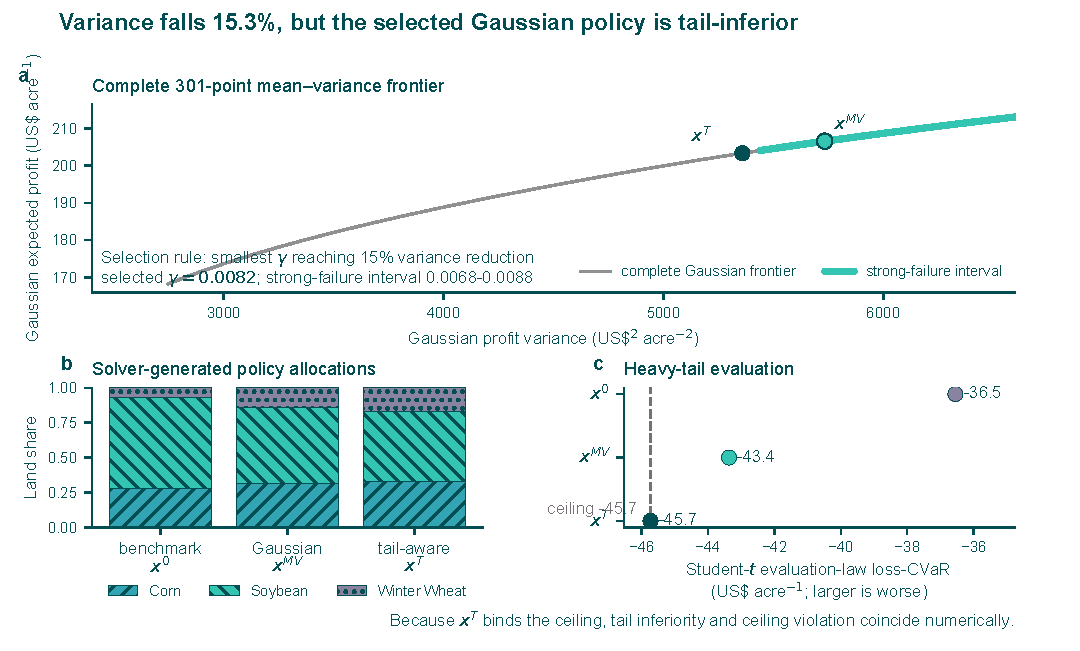
\includegraphics[width=\textwidth]{figures/issue34/Figure3.pdf}
\caption{\textbf{Variance diversification can fail in the joint lower tail.}
\textbf{a}, Gaussian mean--variance and Student-\(t\) CVaR policies use the
same marginals and Kendall's \(\tau\) but choose different crop shares.
\textbf{b}, Gaussian advice exceeds the true-law loss-CVaR ceiling; the
tail-aware policy meets it. \textbf{c}, matched rank dependence does not imply
matched lower-tail dependence.}
\label{fig:diversification}
\end{figure}

\subsection{Policy comparisons and robustness}

The suitability-proportional, winner-take-all and equal-share policies are
projected to operational feasibility before evaluation. Suitability
proportional earns \(\$187.4\) with loss-CVaR \(-\$53.1\) and does not
reverse. Repaired winner-take-all earns \(\$166.6\) with loss-CVaR
\(-\$57.3\) and reverses one pair. Equal share earns \(\$190.4\) with
loss-CVaR \(-\$51.4\). The expected-profit and mean--variance endpoints both
earn \(\$216.5\) but violate the CVaR ceiling. The full model earns less
expected profit than those infeasible endpoints because it buys certified
downside protection.

Every one-at-a-time sensitivity dimension retains selected reversal:
\(\alpha\), constraint regime, dependence family, dependence parameter,
marginal family, sample window, scenario count, seed and solver. Strong
reversal is not universal across every sensitivity cell, which is why the
paper reports selected and strong classifications separately. The solver
comparisons use HiGHS, dual simplex and interior point; scenario counts are
256, 512 and 1,024; sample windows begin in 2016, 2017 or 2018. These
robustness runs assess structural stability, not sampling-independent
replication.

\begin{figure}[t]
\centering
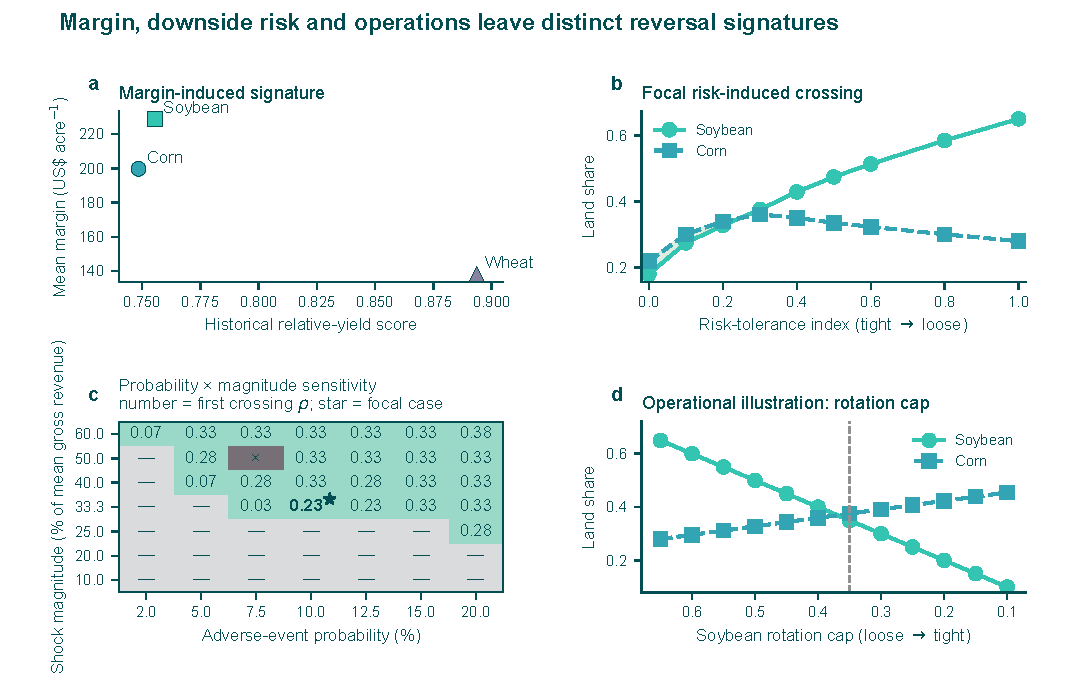
\includegraphics[width=\textwidth]{figures/issue34/Figure4.pdf}
\caption{\textbf{The full model is compared with feasible policy
benchmarks.} \textbf{a}, Repaired score policies, conventional optimization
and the full CVaR policy. \textbf{b}, Expected profit and loss-CVaR reveal
that the highest-profit conventional endpoints lie beyond the registered risk
ceiling. \textbf{c}, Selected reversal persists in every one-at-a-time
robustness dimension.}
\label{fig:policies}
\end{figure}

\subsection{Information and flexibility}

The state proxy is whether the annual Kansas corn-minus-soybean relative-yield
advantage lies below or above its 2016--2023 median. A noisy pre-plant signal
has accuracy 0.5--1.0. The two-stage loss-CVaR restriction is imposed once on
the ex-ante distribution across state, signal and contingent actions; it is
not replaced by a separate risk budget for each signal.

With post-signal acreage reallocation, no adjustable share or an uninformative
signal gives zero value. As accuracy and the adjustable share rise, posterior
allocations diverge and information value reaches
\(\$\,\MaxInformationValue\) per acre. These cells exhibit the action-set
mechanism in the complementarity proposition. With shock buffering, more
flexibility instead contracts state-specific margins toward a common vector.
At perfect signal accuracy, information value declines from approximately
\(\$4.4\) without buffering to numerical zero under full buffering. The
registered grid contains \InfoStrictCells{} strict-complementarity,
\InfoSubCells{} substitution, \InfoZeroCells{} zero and \InfoBoundaryCells{}
boundary cells.

\begin{figure}[t]
\centering
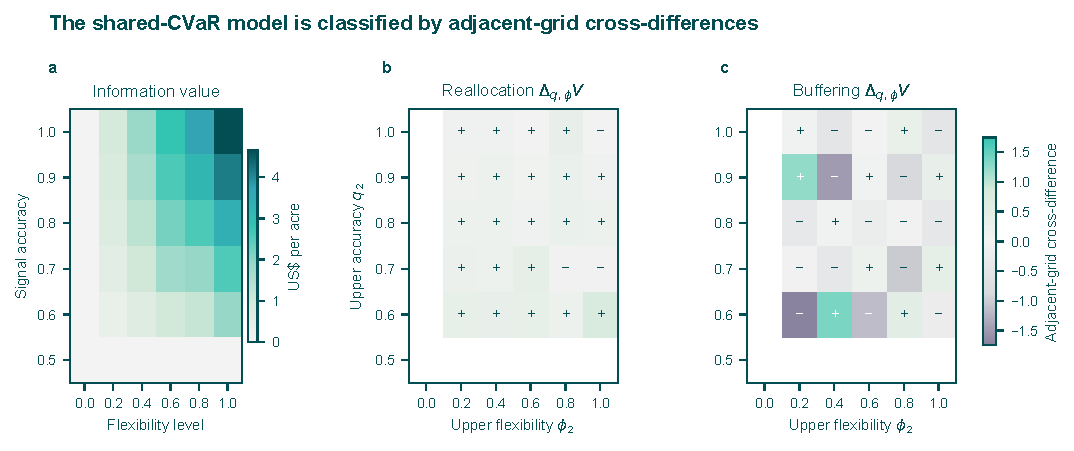
\includegraphics[width=\textwidth]{figures/issue34/Figure5.pdf}
\caption{\textbf{Information value depends on what operational flexibility
can do.} \textbf{a}, A larger post-signal adjustable acreage share makes an
informative signal more actionable. \textbf{b}, Shock-buffering recourse
reduces the payoff difference between predicted states. \textbf{c}, with a
perfect signal, information value falls to zero as buffering fully removes
the state distinction. Values are optimized under one ex-ante loss-CVaR
ceiling.}
\label{fig:information}
\end{figure}

\subsection{Uncertainty}

Sixty-four historical resamples reconstruct score, margins, scenarios and the
full optimum. Reversal probability is \BootstrapProbability{} with 95\%
percentile interval
\([\BootstrapProbabilityLow,\BootstrapProbabilityHigh]\). The first-reversal
risk-tolerance index averages \BootstrapFirstMean{} with interval
\([\BootstrapFirstLow,\BootstrapFirstHigh]\), revealing substantial
uncertainty in the boundary even though reversal itself is common. Mean
bootstrap allocations are 0.277 for corn, 0.527 for soybean and 0.196 for
winter wheat; their percentile intervals are wide because only eight years
enter each calibration. This is the appropriate limitation to emphasize:
the qualitative reversal is stable, while its exact frontier and crop shares
remain imprecise.
